\documentclass[11pt]{article}

\usepackage[margin=1in]{geometry}
\usepackage{amsmath,amssymb,amsthm}
\usepackage{mathpartir}
\usepackage{enumitem}
\usepackage{tikz}
\usetikzlibrary{arrows.meta,positioning,shapes.geometric,fit,backgrounds,calc}
\usepackage{hyperref}
\usepackage[utf8]{inputenc}
\usepackage[T1]{fontenc}
\usepackage{microtype}
\usepackage{xcolor}

\hypersetup{
  colorlinks=true,
  linkcolor=blue!60!black,
  citecolor=green!40!black,
  urlcolor=blue!70!black
}

\theoremstyle{definition}
\newtheorem{definition}{Definition}[section]
\newtheorem{example}{Example}[section]

\theoremstyle{plain}
\newtheorem{theorem}{Theorem}[section]
\newtheorem{lemma}[theorem]{Lemma}

\theoremstyle{remark}
\newtheorem{remark}{Remark}[section]

\newcommand{\hash}{\mathcal{H}}
\newcommand{\hashset}{\mathcal{S}}
\newcommand{\typeindex}{\mathcal{I}}
\newcommand{\namemap}{\mathcal{N}}
\newcommand{\SHA}{\textsf{SHA3}}
\newcommand{\Sort}{\textsf{Sort}}
\newcommand{\Prop}{\textsf{Prop}}
\newcommand{\Type}{\textsf{Type}}
\newcommand{\Nat}{\textsf{Nat}}
\newcommand{\Eq}{\textsf{Eq}}
\newcommand{\bvar}{\textsf{bvar}}
\newcommand{\const}{\textsf{const}}
\newcommand{\app}{\textsf{app}}
\newcommand{\lam}{\textsf{lam}}
\newcommand{\forallE}{\textsf{forallE}}
\newcommand{\letE}{\textsf{letE}}
\newcommand{\concat}{\mathbin{\|}}
\newcommand{\proj}{\textsf{proj}}
\newcommand{\sort}{\textsf{sort}}
\newcommand{\fvar}{\textsf{fvar}}
\newcommand{\mvar}{\textsf{mvar}}
\newcommand{\lit}{\textsf{lit}}
\newcommand{\mdata}{\textsf{mdata}}
\newcommand{\whnf}{\textsf{whnf}}
\newcommand{\Quot}{\textsf{Quot}}

\title{\textbf{HashMath: A Content-Addressed Calculus of Inductive Constructions\\ for Permissionless Formal Mathematics}}
\author{Samuel Schlesinger}
\date{}

\begin{document}
\maketitle

\begin{abstract}
Formalized mathematics is fragmented across incompatible, name-dependent systems.
Lean, Rocq, and Isabelle each maintain curated libraries where every definition and theorem
is identified by a human-chosen name, creating coordination bottlenecks that limit the
scale at which humans and AI can contribute.
We observe that mathematical identity is structural, not nominal: two proof terms with
identical structure are the same proof regardless of what anyone calls them.
We propose \textbf{HashMath}, a content-addressed Calculus of Inductive Constructions (CIC)
in which every well-typed term is indexed by its SHA3 hash, with all dependencies
referenced by hash rather than by name.
The result is a global, permissionless, append-only knowledge base where correctness is
guaranteed by type theory, names are optional metadata, and contributions require
no coordination, review, or naming consensus.
A type-to-inhabitants index enables type-directed search across the entire knowledge base,
allowing AI agents and human mathematicians to discover relevant lemmas by their type
signatures alone.
HashMath provides the infrastructure for Tao's vision of collaborative human-AI mathematics
at scale: 1000 agents and 100 mathematicians contributing simultaneously, building on each
other's work by hash, without a single naming conflict.
\end{abstract}

%% ============================================================
\section{Introduction}
\label{sec:intro}

Formalized mathematics is at an inflection point.
Mathlib, the community-driven library for Lean~4, now contains over 210,000 theorems
and continues to grow at an accelerating pace~\cite{mathlib}.
Google DeepMind's AlphaProof achieved silver-medal performance at the 2024 International
Mathematical Olympiad~\cite{alphaproof}, and DeepSeek-Prover-V2 has reached
gold-level IMO performance~\cite{deepseek}.
Terence Tao envisions a near future in which ``big theorems are proved by 20 people and
multiple AIs, each proving little things''~\cite{tao2025}.

Yet the infrastructure for this vision does not exist.
Today's proof assistants---Lean~\cite{lean4}, Rocq (formerly Coq), Agda, Isabelle/HOL---organize
knowledge through \emph{named references} within \emph{curated repositories}.
Every definition, lemma, and theorem must be given a unique name, reviewed by maintainers,
and placed within a coherent namespace hierarchy.
This works when a small community curates a single library, but it fundamentally limits scale.

\paragraph{The coordination bottleneck.}
Contributing to Mathlib requires conforming to naming conventions, passing linters,
and waiting for human review.
These are reasonable quality controls, but they create a throughput ceiling.
When AI systems can generate thousands of correct proofs per hour, the review queue
becomes the bottleneck, not the proving.
Independent formalizations cannot compose without reconciliation of names, import paths,
and stylistic conventions.

\paragraph{The naming problem.}
Mathematicians disagree on names.
Is it \texttt{Nat.add\_comm} or \texttt{plus\_comm} or \texttt{addition\_commutative}?
Different communities, different languages, and different traditions choose differently.
AI agents, which operate at machine speed, generate names like \texttt{theorem\_7a3f}---functional
but meaningless to humans.
When two independent groups formalize the same theorem under different names, reconciliation
requires human labor to identify the duplication, choose a canonical name, and redirect references.

\paragraph{The Polymath precedent.}
In 2009, Timothy Gowers launched the Polymath project, demonstrating that permissionless
mathematical collaboration works~\cite{gowers2009}.
Over 40 contributors proved the density Hales-Jewett theorem through blog comments, with the
result published in the \emph{Annals of Mathematics}~\cite{polymath2012}.
But the coordination was ad hoc---blog comments, manual tracking, human synthesis.
HashMath provides the infrastructure that Polymath lacked: a system where contributions
compose automatically, correctness is verified mechanically, and no central coordinator is required.

\paragraph{Core insight.}
Mathematical objects have \emph{intrinsic identity} determined by their structure.
The proof that $n + 0 = n$ by induction on $n$ is the same proof regardless of whether
it is called \texttt{Nat.add\_zero}, \texttt{plus\_n\_O}, or \texttt{h\_7f3a2b}.
Names are metadata---useful for human navigation but irrelevant to mathematical content.

We propose \textbf{HashMath}: a content-addressed Calculus of Inductive Constructions in which
every well-typed term is identified by its cryptographic hash.
Dependencies are referenced by hash, not by name.
The result is a global, append-only knowledge base that requires no coordination to use,
no curator to maintain, and no naming consensus to function.

\begin{quote}
\emph{Bitcoin solved double-spending without trusted third parties.
HashMath solves naming conflicts without trusted curators.}
\end{quote}

\begin{figure}[t]
\centering
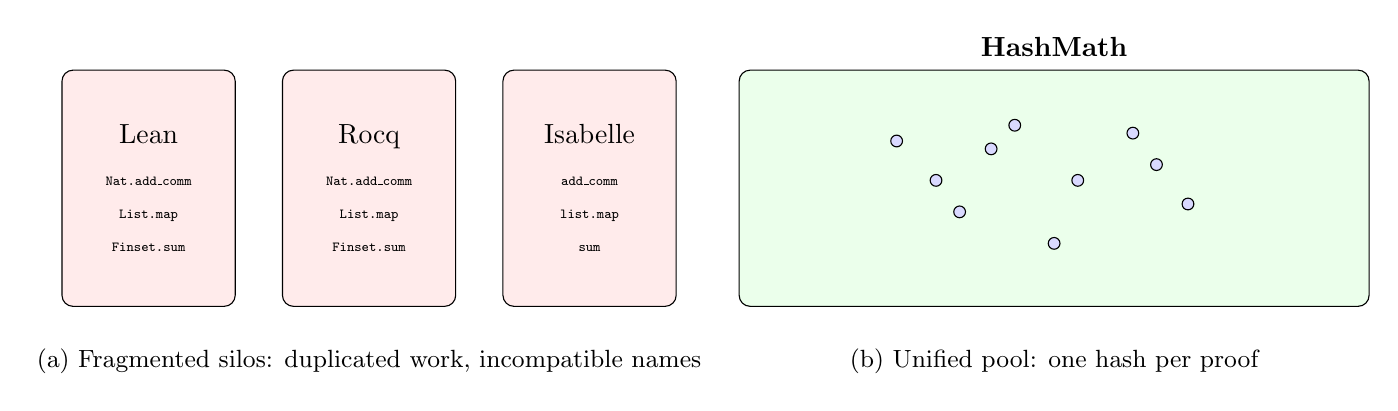
\begin{tikzpicture}[
    silo/.style={draw, rounded corners, minimum width=2.2cm, minimum height=3cm, align=center, fill=red!8},
    pool/.style={draw, rounded corners, minimum width=8cm, minimum height=3cm, align=center, fill=green!8},
    term/.style={draw, circle, inner sep=1.5pt, fill=blue!15, font=\tiny},
    >=Stealth
  ]
  % Silos
  \node[silo] (lean) at (-4, 0) {Lean\\[3pt]\tiny\texttt{Nat.add\_comm}\\\tiny\texttt{List.map}\\\tiny\texttt{Finset.sum}};
  \node[silo] (rocq) at (-1.2, 0) {Rocq\\[3pt]\tiny\texttt{Nat.add\_comm}\\\tiny\texttt{List.map}\\\tiny\texttt{Finset.sum}};
  \node[silo] (isa) at (1.6, 0) {Isabelle\\[3pt]\tiny\texttt{add\_comm}\\\tiny\texttt{list.map}\\\tiny\texttt{sum}};
  \node at (-1.2, -2.2) {\small (a) Fragmented silos: duplicated work, incompatible names};

  % HashMath pool
  \node[pool] (hm) at (7.5, 0) {};
  \node at (7.5, 1.8) {\textbf{HashMath}};
  \foreach \x/\y in {5.5/0.6, 6.3/-0.3, 7.0/0.8, 7.8/0.1, 8.5/0.7, 9.2/-0.2, 6.0/0.1, 7.5/-0.7, 8.8/0.3, 6.7/0.5} {
    \node[term] at (\x, \y) {};
  }
  \node at (7.5, -2.2) {\small (b) Unified pool: one hash per proof};
\end{tikzpicture}
\caption{Formalized mathematics today exists in isolated silos with duplicated effort and incompatible naming.
HashMath provides a single content-addressed pool where every unique proof term has exactly one identity.}
\label{fig:silos}
\end{figure}


%% ============================================================
\section{The Calculus of Inductive Constructions}
\label{sec:cic}

This section gives a precise specification of the \emph{HashMath CIC dialect}---the
subset and variant of the Calculus of Inductive Constructions that HashMath typechecks
and stores.
The dialect is closely aligned with the Lean~4 kernel~\cite{lean4} but strips away
all elaboration-only information (binder names, binder info, free variables, metavariables,
literals, and metadata nodes) so that the core calculus is fully determined by the
mathematical content.
Our presentation follows Coquand and Huet~\cite{coquand1988}, Coquand and
Paulin-Mohring~\cite{coquand1990}, and Werner~\cite{werner1994}, adapted to the
content-addressed setting.

%% --------------------------------------------------
\subsection{Term Constructors}
\label{sec:terms}

Lean~4's kernel defines \texttt{Expr} with 12 constructors.
HashMath retains the 8 constructors that carry type-theoretic content and excludes the
4 that serve only elaboration, metaprogramming, or syntactic sugar.

\begin{definition}[HashMath expression grammar]
\label{def:expr}
HashMath terms are defined by the following grammar:
\[
  e \;\;::=\;\;
    \bvar(n)
    \;\mid\; \sort(u)
    \;\mid\; \const(h, \bar{u})
    \;\mid\; \app(e_1, e_2)
    \;\mid\; \lam(e_T, e_b)
    \;\mid\; \forallE(e_T, e_b)
    \;\mid\; \letE(e_T, e_v, e_b)
    \;\mid\; \proj(h, i, e)
\]
where $n \in \mathbb{N}$, $u$ is a universe level (Section~\ref{sec:levels}),
$h \in \{0,1\}^{256}$ is a content hash, $\bar{u}$ is a list of universe levels,
and $i \in \mathbb{N}$.
\end{definition}

The constructors are:
\begin{itemize}[nosep]
  \item $\bvar(n)$ --- a de Bruijn bound variable with index $n$.
  \item $\sort(u)$ --- a universe sort at level $u$; $\sort(\textsf{zero})$ is $\Prop$ and $\sort(\textsf{succ}(n))$ is $\Type(n)$.
  \item $\const(h, \bar{u})$ --- a reference to a previously declared constant identified by its content hash $h$, instantiated at universe levels $\bar{u}$.
        Crucially, constants are referenced \emph{by hash}, not by name.
  \item $\app(e_1, e_2)$ --- function application.
  \item $\lam(e_T, e_b)$ --- lambda abstraction with domain type $e_T$ and body $e_b$.
        Binder name and binder info (implicit/explicit/instance) are \emph{excluded}: they are elaboration metadata, not type-theoretic content.
  \item $\forallE(e_T, e_b)$ --- dependent product $\Pi$-type with domain $e_T$ and codomain $e_b$.
        Binder name and binder info are again excluded.
  \item $\letE(e_T, e_v, e_b)$ --- let binding with type annotation $e_T$, value $e_v$, and body $e_b$.
        Binder name is excluded.
  \item $\proj(h, i, e)$ --- projection of the $i$-th field from a structure whose inductive type has hash $h$, applied to term $e$.
\end{itemize}

\paragraph{Excluded constructors.}
Table~\ref{tab:constructors} summarizes the status of all 12 Lean~4 \texttt{Expr}
constructors.
The four excluded constructors are:
\begin{itemize}[nosep]
  \item $\fvar$ (free variables) --- HashMath stores only \emph{closed} terms; all variables under consideration are bound.
  \item $\mvar$ (metavariables) --- placeholders for the elaborator; absent from fully elaborated kernel terms.
  \item $\lit$ (literals) --- Lean~4 uses $\lit$ for efficient \texttt{Nat} and \texttt{String} literals. These are syntactic sugar that can always be expanded to the corresponding constructor applications ($\textsf{succ}(\textsf{succ}(\cdots))$ for natural numbers, a list of characters for strings).
        HashMath requires the expanded form.
  \item $\mdata$ (metadata) --- annotation nodes carrying elaboration metadata. These have no type-theoretic content and are stripped.
\end{itemize}

\begin{table}[t]
\centering
\begin{tabular}{llcl}
\hline
\textbf{Lean 4 Constructor} & \textbf{Purpose} & \textbf{HashMath} & \textbf{Notes} \\
\hline
\texttt{bvar}    & Bound variable       & \checkmark & De Bruijn index \\
\texttt{fvar}    & Free variable        & ---        & Only closed terms stored \\
\texttt{mvar}    & Metavariable         & ---        & Elaboration only \\
\texttt{sort}    & Universe sort        & \checkmark & \\
\texttt{const}   & Named constant       & \checkmark & By hash, not name \\
\texttt{app}     & Application          & \checkmark & \\
\texttt{lam}     & Lambda               & \checkmark & Name + info excluded \\
\texttt{forallE} & Dependent product    & \checkmark & Name + info excluded \\
\texttt{letE}    & Let binding          & \checkmark & Name excluded \\
\texttt{lit}     & Literal              & ---        & Expand to constructors \\
\texttt{mdata}   & Metadata             & ---        & Elaboration only \\
\texttt{proj}    & Projection           & \checkmark & \\
\hline
\end{tabular}
\caption{Lean~4 \texttt{Expr} constructors and their status in HashMath.
  Of the 12 constructors, 8 are retained (type-theoretic content) and 4 are
  excluded (elaboration or syntactic sugar).}
\label{tab:constructors}
\end{table}

%% --------------------------------------------------
\subsection{Universe Levels}
\label{sec:levels}

Universe levels govern the stratification of types.

\begin{definition}[Level]
\label{def:level}
The type of universe levels is defined by:
\[
  u \;\;::=\;\;
    \textsf{zero}
    \;\mid\; \textsf{succ}(u)
    \;\mid\; \max(u_1, u_2)
    \;\mid\; \textsf{imax}(u_1, u_2)
    \;\mid\; \textsf{param}(n)
\]
where $n \in \mathbb{N}$ is a de Bruijn index into the list of universe parameters
of the enclosing declaration.
\end{definition}

The constructors are:
\begin{itemize}[nosep]
  \item $\textsf{zero}$ --- the base level.
  \item $\textsf{succ}(u)$ --- the successor of level $u$.
  \item $\max(u_1, u_2)$ --- the maximum of two levels.
  \item $\textsf{imax}(u_1, u_2)$ --- the \emph{impredicative maximum}: $\textsf{imax}(u_1, u_2)$ equals $\textsf{zero}$ if $u_2$ evaluates to $\textsf{zero}$, and $\max(u_1, u_2)$ otherwise.
        This is essential for typing $\Pi$-types into $\Prop$ (see Section~\ref{sec:typing}).
  \item $\textsf{param}(n)$ --- a universe parameter variable, referenced by de Bruijn index rather than by name, for the same content-addressing reasons that binder names are excluded from terms.
\end{itemize}

\paragraph{Excluded constructor.}
Lean~4's \texttt{Level} type also has a \texttt{mvar} constructor for universe metavariables.
These are elaboration-time placeholders and are excluded from HashMath, just as expression
metavariables are excluded.

%% --------------------------------------------------
\subsection{Typing Rules}
\label{sec:typing}

A context $\Gamma$ is a list of typed variable declarations.
The judgment $\Gamma \vdash e : T$ asserts that term $e$ has type $T$ in context $\Gamma$.

\begin{mathpar}
  \inferrule*[Right=Sort]
    { }
    {\Gamma \vdash \sort(u) : \sort(\textsf{succ}(u))}

  \inferrule*[Right=Var]
    {\Gamma(n) = T}
    {\Gamma \vdash \bvar(n) : T}

  \inferrule*[Right=Pi]
    {\Gamma \vdash A : \sort(i) \\ \Gamma, A \vdash B : \sort(j)}
    {\Gamma \vdash \forallE(A, B) : \sort(\textsf{imax}(i,j))}
\end{mathpar}

\begin{mathpar}
  \inferrule*[Right=Lam]
    {\Gamma \vdash A : \sort(i) \\ \Gamma, A \vdash t : B}
    {\Gamma \vdash \lam(A, t) : \forallE(A, B)}

  \inferrule*[Right=App]
    {\Gamma \vdash f : \forallE(A, B) \\ \Gamma \vdash a : A}
    {\Gamma \vdash \app(f, a) : B[a/0]}

  \inferrule*[Right=Let]
    {\Gamma \vdash T : \sort(u) \\ \Gamma \vdash v : T \\ \Gamma, T \vdash b : B}
    {\Gamma \vdash \letE(T, v, b) : B[v/0]}
\end{mathpar}

\begin{mathpar}
  \inferrule*[Right=Const]
    {\textsf{decl}(h) = (k, \tau) \\ |\bar{u}| = k}
    {\Gamma \vdash \const(h, \bar{u}) : \tau[\bar{u}]}

  \inferrule*[Right=Conv]
    {\Gamma \vdash e : T \\ T \equiv T'}
    {\Gamma \vdash e : T'}
\end{mathpar}

Several points deserve emphasis:

\paragraph{Sort rule for $\Pi$-types.}
The sort of $\forallE(A, B)$ uses $\textsf{imax}(i, j)$ rather than $\max(i, j)$.
When $B : \Prop$ (i.e., $j = 0$), the product type also lives in $\Prop$ regardless
of the level of $A$.
This is what makes $\Prop$ impredicative: one can quantify over all types and still
land in $\Prop$.

\paragraph{Cumulativity.}
The universe hierarchy is cumulative:
\[
  \Prop \leq \Type(0) \leq \Type(1) \leq \Type(2) \leq \cdots
\]
If $\Gamma \vdash e : \sort(u)$ and $u \leq u'$, then $\Gamma \vdash e : \sort(u')$.
Cumulativity is built into the conversion rule: the definitional equality check $T \equiv T'$
accounts for subtyping of sorts.

\paragraph{De Bruijn conventions.}
Since binder names are absent, contexts are lists rather than named mappings, and
substitution $B[a/0]$ replaces de Bruijn index 0 and shifts remaining indices.
The notation $\Gamma, A$ extends the context with a new variable of type $A$ at index 0.

%% --------------------------------------------------
\subsection{Reductions}
\label{sec:reductions}

Definitional equality $\equiv$ is generated by the following reduction rules:

\begin{itemize}[nosep]
  \item \textbf{$\beta$-reduction}: $\app(\lam(A, t),\; a) \;\longrightarrow_\beta\; t[a/0]$

  \item \textbf{$\delta$-reduction}: unfold a constant to its definition.
        If $\textsf{decl}(h)$ is a definition with value $v$, then $\const(h, \bar{u}) \;\longrightarrow_\delta\; v[\bar{u}]$.
        In HashMath, \emph{all definitions are always transparent}: there is no opacity mechanism (see Section~\ref{sec:transparency}).

  \item \textbf{$\iota$-reduction}: a recursor applied to a constructor computes.
        If $\textsf{rec}_I$ is the recursor for inductive type $I$ and $c_k$ is the $k$-th constructor,
        then $\textsf{rec}_I \; \bar{p} \; \bar{m} \; (c_k \; \bar{p} \; \bar{a}) \;\longrightarrow_\iota\; m_k \; \bar{a}$
        (where $\bar{p}$ are parameters, $\bar{m}$ are motives and minor premises, and $m_k$ is the minor premise for $c_k$).

  \item \textbf{$\zeta$-reduction}: substitute let bindings.
        $\letE(T, v, b) \;\longrightarrow_\zeta\; b[v/0]$

  \item \textbf{Projection reduction}: $\proj(h_I, i, c_k \; \bar{p} \; \bar{a}) \;\longrightarrow\; a_i$,
        where $c_k$ is the single constructor of the structure $I$ and $a_i$ is the $i$-th field argument.

  \item \textbf{Quotient reduction}: The Quot type (Section~\ref{sec:quotient}) has two computation rules:
        \begin{align*}
          \Quot.\textsf{lift}\; f\; h\; (\Quot.\textsf{mk}\; r\; a) &\;\longrightarrow\; f\; a \\
          \Quot.\textsf{ind}\; \varphi\; h\; (\Quot.\textsf{mk}\; r\; a) &\;\longrightarrow\; \varphi\; a
        \end{align*}
\end{itemize}

In addition to these reduction rules, definitional equality includes the following
equivalences:

\begin{itemize}[nosep]
  \item \textbf{$\eta$-equivalence}: $f \equiv \lam(A, \app(f', \bvar(0)))$ where $f'$ is $f$ with de Bruijn indices shifted up by 1, provided $f : \forallE(A, B)$.

  \item \textbf{Proof irrelevance for $\Prop$}: if $p, q : T$ and $T : \Prop$, then $p \equiv q$.
        All proofs of a proposition are definitionally equal.

  \item \textbf{Structural $\eta$ for structures}: if $I$ is a structure (a single-constructor inductive with no indices) and $s : I \; \bar{p}$, then
        $s \equiv c(\bar{p}, \proj(h_I, 0, s), \proj(h_I, 1, s), \ldots, \proj(h_I, n{-}1, s))$
        where $c$ is the unique constructor.
\end{itemize}

CIC enjoys the property that definitional equality is decidable, which is essential for
typechecking to be decidable.

%% --------------------------------------------------
\subsection{Definitional Equality Algorithm}
\label{sec:defeq}

The definitional equality check $e_1 \equiv e_2$ is the heart of the typechecker.
We outline the algorithm, which follows the Lean~4 kernel~\cite{lean4} with the
simplification that there is no opacity to manage.

\begin{enumerate}[nosep]
  \item \textbf{Syntactic equality.}
        If $e_1$ and $e_2$ are syntactically identical (same AST), return true.
        This short-circuits the common case.

  \item \textbf{Weak-head normalization (core).}
        Reduce both sides using $\whnf_{\textsf{core}}$, which applies $\beta$, $\zeta$, $\iota$, projection, and quotient reductions---but \emph{not} $\delta$.
        Deferring $\delta$-reduction avoids expensive unfolding when possible.

  \item \textbf{Syntactic equality after $\whnf_{\textsf{core}}$.}
        Compare the reduced terms. If equal, return true.

  \item \textbf{Proof irrelevance.}
        If both sides have a type in $\Prop$, return true.

  \item \textbf{$\delta$-reduction.}
        Unfold constants on both sides (in HashMath, all constants are transparent) and repeat the comparison.
        When both sides are constants, a heuristic unfolds the ``simpler'' side first.

  \item \textbf{Constant equality.}
        If both sides are $\const(h_1, \bar{u}_1)$ and $\const(h_2, \bar{u}_2)$ with $h_1 = h_2$, check that $\bar{u}_1$ and $\bar{u}_2$ are pointwise equal as levels.

  \item \textbf{Application congruence.}
        If both sides are applications $\app(f_1, a_1)$ and $\app(f_2, a_2)$,
        recursively check $f_1 \equiv f_2$ and $a_1 \equiv a_2$.

  \item \textbf{$\eta$-expansion.}
        If one side is $\lam(A, b)$ and the other is not, $\eta$-expand the non-lambda side and recurse.

  \item \textbf{Structural $\eta$.}
        If both sides have a structure type, project all fields and compare pairwise.
\end{enumerate}

If none of these steps succeeds, the terms are not definitionally equal.

%% --------------------------------------------------
\subsection{Declaration Kinds}
\label{sec:declarations}

Every entry in the HashMath store is a \emph{declaration}.
There are four kinds:

\begin{definition}[Declaration]
\label{def:decl}
A declaration is one of:
\begin{itemize}[nosep]
  \item $\textsf{axiom}(k, \tau)$ --- an axiom with $k$ universe parameters and type $\tau$.
        No definition body; the axiom is trusted.
  \item $\textsf{definition}(k, \tau, v)$ --- a definition with $k$ universe parameters, type $\tau$, and value $v$.
        The typechecker verifies $v : \tau$.
  \item $\textsf{inductive}(\mathit{block})$ --- an inductive type declaration (see Section~\ref{sec:inductive}).
  \item $\textsf{quotient}(\mathit{kind})$ --- one of the four built-in quotient constants (see Section~\ref{sec:quotient}).
\end{itemize}
\end{definition}

In all cases, $k \in \mathbb{N}$ specifies the number of universe parameters.
The type $\tau$ and value $v$ (when present) may contain $\textsf{param}(n)$ level
expressions for $0 \leq n < k$.

%% --------------------------------------------------
\subsection{Inductive Types}
\label{sec:inductive}

An inductive type declaration specifies a family of mutually defined types and their constructors.
The \emph{strict positivity} constraint ensures that recursive occurrences of the type being defined
appear only in strictly positive positions in constructor argument types, guaranteeing logical consistency~\cite{paulin1993}.

\begin{definition}[Inductive block]
\label{def:inductive-block}
An inductive block is a record:
\[
  \textsf{InductiveBlock} \;=\; \{
    k \in \mathbb{N},\;
    p \in \mathbb{N},\;
    \mathit{types} : \textsf{List}\;\textsf{InductiveType},\;
    \mathit{isUnsafe} : \textsf{Bool}
  \}
\]
where $k$ is the number of universe parameters, $p$ is the number of parameters, and each
$\textsf{InductiveType}$ is:
\[
  \textsf{InductiveType} \;=\; \{
    \mathit{type} : \textsf{Expr},\;
    \mathit{ctors} : \textsf{List}\;\textsf{Expr}
  \}
\]
The $\mathit{type}$ field gives the type former's type, and $\mathit{ctors}$ lists the types
of each constructor.
Mutual inductive types have multiple entries in $\mathit{types}$.
\end{definition}

\begin{example}[Natural numbers]
The natural numbers are defined inductively:
\[
  \textsf{InductiveBlock}\{k=0,\; p=0,\;
    \mathit{types} = [\{
      \mathit{type} = \Type,\;
      \mathit{ctors} = [\Nat,\; \Nat \to \Nat]
    \}],\;
    \mathit{isUnsafe} = \textsf{false}\}
\]
Here $\Nat : \Type$ is the type former, and the two constructors have types
$\textsf{zero} : \Nat$ and $\textsf{succ} : \Nat \to \Nat$.
The elimination principle (recursor) is generated automatically.
\end{example}

\begin{example}[Propositional equality]
The identity type $\Eq$ is an inductive family with $k=1$ universe parameter and $p=1$ parameter:
\[
  \textsf{InductiveBlock}\{k=1,\; p=1,\;
    \mathit{types} = [\{
      \mathit{type} = \Pi(A{:}\Type_u).\,A \to A \to \Prop,\;
      \mathit{ctors} = [\Pi(A{:}\Type_u).\,\Pi(a{:}A).\,\Eq\;A\;a\;a]
    \}],\;
    \mathit{isUnsafe} = \textsf{false}\}
\]
\end{example}

%% --------------------------------------------------
\subsection{Quotient Types}
\label{sec:quotient}

Lean~4 (and therefore HashMath) includes four built-in constants for quotient types, which
cannot be defined as ordinary inductive types:

\begin{itemize}[nosep]
  \item $\Quot : (\alpha : \Sort(u)) \to (\alpha \to \alpha \to \Prop) \to \Sort(u)$ --- the quotient type former.
  \item $\Quot.\textsf{mk} : \{r : \alpha \to \alpha \to \Prop\} \to \alpha \to \Quot\;\alpha\;r$ --- the quotient constructor.
  \item $\Quot.\textsf{lift} : ((\alpha \to \beta) \to (\forall\;a\;b,\; r\;a\;b \to f\;a = f\;b) \to \Quot\;\alpha\;r \to \beta)$ --- lift a function that respects the equivalence relation.
  \item $\Quot.\textsf{ind} : (\forall\;a,\; \varphi\;(\Quot.\textsf{mk}\;r\;a)) \to \forall\;q,\; \varphi\;q$ --- the induction principle.
\end{itemize}

The $\mathit{kind}$ field in a quotient declaration identifies which of these four constants it is.
Their computation rules are given in Section~\ref{sec:reductions}.

%% --------------------------------------------------
\subsection{Universe Polymorphism}
\label{sec:universes}

Modern implementations of CIC (including Lean~4) support \emph{universe polymorphism}:
definitions can be parameterized by universe level variables, instantiated at each use site.
This avoids code duplication and is essential for a practical foundation.

The universe hierarchy is:
\[
  \Prop \;:\; \Type(0) \;:\; \Type(1) \;:\; \Type(2) \;:\; \cdots
\]
Universe levels are compared using the normalization procedure: reduce $\max$ and $\textsf{imax}$
where possible, then check pointwise equality of the resulting normal forms.
Universe polymorphism interacts importantly with content-addressing (Section~\ref{sec:hash-universes}).

\begin{figure}[t]
\centering
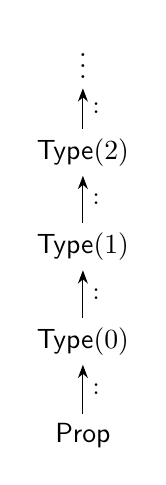
\begin{tikzpicture}[>=Stealth, node distance=1.2cm]
  \node (prop) {\(\Prop\)};
  \node[above of=prop] (t0) {\(\Type(0)\)};
  \node[above of=t0] (t1) {\(\Type(1)\)};
  \node[above of=t1] (t2) {\(\Type(2)\)};
  \node[above of=t2] (dots) {\(\vdots\)};
  \draw[->] (prop) -- node[right, font=\small] {:} (t0);
  \draw[->] (t0) -- node[right, font=\small] {:} (t1);
  \draw[->] (t1) -- node[right, font=\small] {:} (t2);
  \draw[->] (t2) -- node[right, font=\small] {:} (dots);
\end{tikzpicture}
\caption{The universe hierarchy. Each sort inhabits the next, forming a cumulative tower.
$\Prop$ is impredicative: $\Pi$-types into $\Prop$ remain in $\Prop$.}
\label{fig:universes}
\end{figure}

%% --------------------------------------------------
\subsection{Transparency Model}
\label{sec:transparency}

In Lean~4, definitions carry an opacity attribute (\texttt{@[reducible]},
\texttt{@[semireducible]}, \texttt{@[irreducible]}) that controls when the
definitional equality checker may unfold them.
This is an important performance optimization for a practical proof assistant but
introduces an elaboration-level concern into the kernel: two terms may or may not
be definitionally equal depending on the transparency setting.

HashMath takes a simpler approach: \textbf{all definitions are always fully transparent}.
The definitional equality checker may unfold any definition at any time.
There is no opacity mechanism.

This simplification is justified by the content-addressing design:
\begin{itemize}[nosep]
  \item Opacity is a \emph{performance} concern, not a \emph{correctness} concern.
        A term that typechecks with some definitions opaque also typechecks with all definitions transparent (though possibly more slowly).
  \item Content-addressing requires a canonical notion of definitional equality.
        If opacity affected which terms are equal, two verifiers with different opacity settings might disagree, breaking the determinism that content-addressing requires.
  \item The absence of opacity simplifies the kernel and the definitional equality algorithm.
\end{itemize}


%% ============================================================
\section{Content-Addressed Terms}
\label{sec:content}

\subsection{The Naming Problem in Detail}
\label{sec:naming-problem}

Consider the theorem that addition on natural numbers is commutative.
In Lean~4's Mathlib, this is \texttt{Nat.add\_comm}.
In Rocq's standard library, it is also \texttt{Nat.add\_comm}---but the two are not interchangeable
because they exist in different systems with different elaboration, different dependencies, and
different internal representations.
An AI agent might prove the same theorem and call it \texttt{theorem\_7a3f}.
Three correct formalizations of the same mathematical fact, none of which can reference the others.

The problem compounds at scale.
Mathlib has undergone multiple renaming campaigns, where thousands of theorems are renamed
to conform to evolving conventions.
Each renaming breaks downstream projects that depend on the old names.
When independent groups formalize overlapping mathematics, reconciliation requires human labor
to identify duplicates, choose canonical names, and redirect references.

\subsection{Content-Addressing for CIC Terms}
\label{sec:hashing}

We define the hash function $\hash$ on CIC terms at the byte level.
All hashing uses SHA3-256~\cite{sha3}.
Single-byte tags provide domain separation between constructors, natural numbers are
encoded as unsigned LEB128, and hashes are fixed 32-byte values.
This specification is complete and unambiguous---it uniquely determines the hash of
every well-formed term, level, and declaration.

\begin{definition}[Level hash]
\label{def:hash-level}
The hash of a universe level is:
\begin{align*}
  \hash(\textsf{zero}) &= \SHA(\mathtt{0x00}) \\
  \hash(\textsf{succ}(l)) &= \SHA(\mathtt{0x01} \concat \hash(l)) \\
  \hash(\textsf{max}(l_1, l_2)) &= \SHA(\mathtt{0x02} \concat \hash(l_1) \concat \hash(l_2)) \\
  \hash(\textsf{imax}(l_1, l_2)) &= \SHA(\mathtt{0x03} \concat \hash(l_1) \concat \hash(l_2)) \\
  \hash(\textsf{param}(n)) &= \SHA(\mathtt{0x04} \concat \textsf{leb128}(n))
\end{align*}
\end{definition}

\begin{definition}[Term hash]
\label{def:hash}
The hash function $\hash : \textsf{Expr} \to \{0,1\}^{256}$ is:
\begin{align*}
  \hash(\bvar(n)) &= \SHA(\mathtt{0x10} \concat \textsf{leb128}(n)) \\
  \hash(\Sort(l)) &= \SHA(\mathtt{0x11} \concat \hash(l)) \\
  \hash(\const(h, [l_0, \ldots, l_{n-1}])) &= \SHA(\mathtt{0x12} \concat h \concat \textsf{leb128}(n) \concat \hash(l_0) \concat \cdots \concat \hash(l_{n-1})) \\
  \hash(\app(f, a)) &= \SHA(\mathtt{0x13} \concat \hash(f) \concat \hash(a)) \\
  \hash(\lam(T, b)) &= \SHA(\mathtt{0x14} \concat \hash(T) \concat \hash(b)) \\
  \hash(\forallE(T, b)) &= \SHA(\mathtt{0x15} \concat \hash(T) \concat \hash(b)) \\
  \hash(\letE(T, v, b)) &= \SHA(\mathtt{0x16} \concat \hash(T) \concat \hash(v) \concat \hash(b)) \\
  \hash(\textsf{proj}(h, i, e)) &= \SHA(\mathtt{0x17} \concat h \concat \textsf{leb128}(i) \concat \hash(e))
\end{align*}
where $h$ in $\const$ and $\textsf{proj}$ is the 32-byte hash of the referenced declaration,
and $\textsf{leb128}$ denotes unsigned LEB128 encoding.
Binder names and binder info are excluded: only the type-theoretic content is hashed.
\end{definition}

\begin{definition}[Declaration hash]
\label{def:hash-decl}
The hash of a declaration is:
\begin{align*}
  \hash(\textsf{axiom}(n, T)) &= \SHA(\mathtt{0x20} \concat \textsf{leb128}(n) \concat \hash(T)) \\
  \hash(\textsf{definition}(n, T, v)) &= \SHA(\mathtt{0x21} \concat \textsf{leb128}(n) \concat \hash(T) \concat \hash(v)) \\
  \hash(\textsf{inductive}(\textit{block})) &= \SHA(\mathtt{0x22} \concat \textsf{encode}(\textit{block})) \\
  \hash(\textsf{quotient}(k)) &= \SHA(\mathtt{0x23} \concat k_{\textsf{byte}})
\end{align*}
where $n$ is the number of universe parameters and the inductive block encoding follows
the same conventions (LEB128 lengths, recursive sub-hashing).
\end{definition}

\begin{remark}
The tag bytes are chosen so that levels (\texttt{0x00}--\texttt{0x04}),
expressions (\texttt{0x10}--\texttt{0x17}), and declarations (\texttt{0x20}--\texttt{0x23})
occupy disjoint ranges.
This ensures that no term can collide with a level or declaration at the SHA3 input level,
even before considering structural differences.
\end{remark}

Several design decisions are critical:

\paragraph{Binder names and binder info are excluded.}
The terms $\lambda(x{:}\Nat).\,x$ and $\lambda(y{:}\Nat).\,y$ are $\alpha$-equivalent
and receive the same hash, since both have de Bruijn representation
$\lam(\Nat, \bvar(0))$.
Lean~4's binder info (implicit, explicit, instance) is an elaboration concern
and is similarly excluded.

\paragraph{Constants reference by hash.}
The hash of $\const(h, \bar{u})$ includes the 32-byte hash $h$ of the referenced declaration.
This is the key move that eliminates name-dependence: two constants with different names but
identical definitions produce the same hash.

\paragraph{Free variables are forbidden.}
Only \emph{closed} terms---those with no free variables---may be stored in the hashset.
Every bound variable must be under a binder, and every constant must resolve to a stored definition.

\begin{example}[Hashing the identity function on $\Nat$]
\label{ex:identity}
Consider $\lambda(n{:}\Nat).\,n$, which in de Bruijn notation is $\lam(\Nat, \bvar(0))$.
Its hash is:
\[
  \hash(\lam(\Nat, \bvar(0))) = \SHA(\mathtt{0x14} \concat \hash(\Nat) \concat \SHA(\mathtt{0x10} \concat \textsf{leb128}(0)))
\]
where $\hash(\Nat)$ is the hash of the inductive declaration defining $\Nat$.
\end{example}

\begin{example}[Alpha-equivalence]
\label{ex:alpha}
The terms $\lambda(x{:}\Nat).\,x$ and $\lambda(y{:}\Nat).\,y$ both have de Bruijn representation
$\lam(\Nat, \bvar(0))$.
Since binder names are excluded from the hash, they produce identical hashes. \qed
\end{example}

\subsection{Capturing the Environment}
\label{sec:hash-closure}

\begin{definition}[Hash-closed term]
A term $t$ is \emph{hash-closed} if every constant reference $\const(n, \bar{u})$ occurring
in $t$ can be resolved to a declaration whose hash exists in the hashset $\hashset$.
\end{definition}

Hash-closure means that the hash of any term transitively encodes its entire dependency tree.
This creates a \textbf{Merkle DAG} of mathematical knowledge: the hash of \texttt{Nat.add\_comm}
encodes, through the hashes of its subterms, the definitions of $\Nat$, $\Nat.\textsf{add}$, $\Eq$,
and transitively down to the axioms of the type theory.

\begin{figure}[t]
\centering
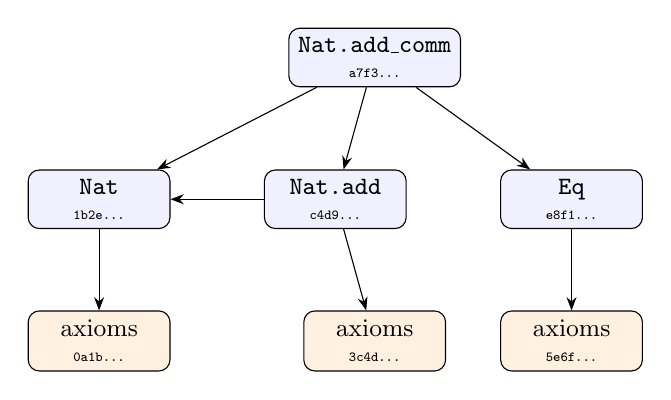
\begin{tikzpicture}[
    node/.style={draw, rounded corners, font=\small, fill=blue!6, minimum width=1.8cm, align=center},
    axiom/.style={draw, rounded corners, font=\small, fill=orange!12, minimum width=1.8cm, align=center},
    >=Stealth
  ]
  \node[node] (addcomm) at (0, 0) {\texttt{Nat.add\_comm}\\[-2pt]\tiny\texttt{a7f3...}};
  \node[node] (nat) at (-3.5, -1.8) {\texttt{Nat}\\[-2pt]\tiny\texttt{1b2e...}};
  \node[node] (add) at (-0.5, -1.8) {\texttt{Nat.add}\\[-2pt]\tiny\texttt{c4d9...}};
  \node[node] (eq) at (2.5, -1.8) {\texttt{Eq}\\[-2pt]\tiny\texttt{e8f1...}};
  \node[axiom] (ax1) at (-3.5, -3.6) {axioms\\[-2pt]\tiny\texttt{0a1b...}};
  \node[axiom] (ax2) at (0, -3.6) {axioms\\[-2pt]\tiny\texttt{3c4d...}};
  \node[axiom] (ax3) at (2.5, -3.6) {axioms\\[-2pt]\tiny\texttt{5e6f...}};

  \draw[->] (addcomm) -- (nat);
  \draw[->] (addcomm) -- (add);
  \draw[->] (addcomm) -- (eq);
  \draw[->] (nat) -- (ax1);
  \draw[->] (add) -- (nat);
  \draw[->] (add) -- (ax2);
  \draw[->] (eq) -- (ax3);
\end{tikzpicture}
\caption{Merkle DAG of \texttt{Nat.add\_comm}. Each node's hash transitively encodes all dependencies
down to the axioms. Human-readable names shown for clarity; the system operates on hashes.}
\label{fig:merkle}
\end{figure}

\subsection{Mutual Recursive Definitions}
\label{sec:mutual}

Mutual recursion presents a challenge: if definition $A$ references $B$ and $B$ references $A$,
then $\hash(A)$ depends on $\hash(B)$ and vice versa.

\begin{definition}[Mutual block hash]
A mutual recursive block $M = (d_1, \ldots, d_k)$ is an ordered list of definitions that
may reference each other.
The block hash is:
\[
  \hash(M) = \SHA(\texttt{"mutual"} \concat \hash_{\textsf{raw}}(d_1) \concat \cdots \concat \hash_{\textsf{raw}}(d_k))
\]
where $\hash_{\textsf{raw}}(d_i)$ hashes definition $d_i$ with intra-block references represented
as block-relative indices rather than hashes.
Each individual definition's identity is then the pair $(\hash(M), i)$ where $i$ is its index
within the block.
\end{definition}

This is analogous to how Lean~4 handles \texttt{mutual ... end} blocks.
The approach preserves the acyclic Merkle DAG property at the block level: blocks reference
other blocks (or individual definitions), and no cyclic block dependencies are permitted.

\subsection{The Global Hashset}
\label{sec:hashset}

\begin{definition}[Hashset]
The global hashset is a set of verified triples:
\[
  \hashset = \{ (h, t, T) \mid h = \hash(t),\; T = \textsf{typeof}(t),\; \textsf{well\_typed}(t) \}
\]
together with a \emph{type index}:
\[
  \typeindex : \{0,1\}^{256} \to \mathcal{P}(\{0,1\}^{256}), \qquad
  \typeindex(h_T) = \{ h \mid (h, t, T) \in \hashset,\; \hash(T) = h_T \}
\]
mapping each type hash to the set of hashes of its inhabitants.
\end{definition}

The hashset is \emph{append-only}: once a verified triple is added, it is never removed.
Since well-typedness is verified before insertion, every entry in the hashset is correct by construction.

\begin{figure}[t]
\centering
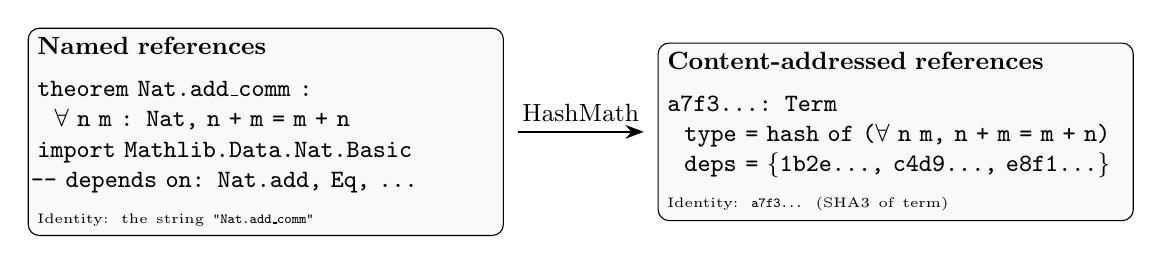
\begin{tikzpicture}[
    box/.style={draw, rounded corners, font=\small, align=left, fill=gray!5, text width=5.8cm},
    >=Stealth
  ]
  \node[box] (named) at (-4, 0) {
    \textbf{Named references}\\[4pt]
    \texttt{theorem Nat.add\_comm :}\\
    \texttt{~~$\forall$ n m : Nat, n + m = m + n}\\
    \texttt{import Mathlib.Data.Nat.Basic}\\
    \texttt{-- depends on: Nat.add, Eq, ...}\\[2pt]
    {\tiny Identity: the string \texttt{"Nat.add\_comm"}}
  };
  \node[box] (hashed) at (4, 0) {
    \textbf{Content-addressed references}\\[4pt]
    \texttt{a7f3...: Term}\\
    \texttt{~~type = hash of ($\forall$ n m, n + m = m + n)}\\
    \texttt{~~deps = \{1b2e..., c4d9..., e8f1...\}}\\[2pt]
    {\tiny Identity: \texttt{a7f3...} (SHA3 of term)}
  };
  \draw[->, thick] (-0.8, 0) -- (0.8, 0) node[midway, above, font=\small] {HashMath};
\end{tikzpicture}
\caption{Named references (left) identify terms by human-chosen strings within a specific library.
Content-addressed references (right) identify terms by their cryptographic hash, independent of any naming convention.}
\label{fig:named-vs-hashed}
\end{figure}

\subsection{Comparison with Unison}
\label{sec:unison}

The Unison programming language pioneered content-addressing for general-purpose code,
hashing abstract syntax trees with 512-bit SHA3~\cite{unison}.
HashMath adapts this approach for the specific demands of formal mathematics:

\begin{itemize}[nosep]
  \item \textbf{Type-to-inhabitants index}: Unison does not maintain a global map from types
    to their inhabitants, because general-purpose code does not have the same ``search by type'' need.
  \item \textbf{Formal verification}: every term in HashMath is type-checked before insertion;
    Unison stores arbitrary well-scoped code without a comparable verification step.
  \item \textbf{Universe polymorphism}: CIC's universe polymorphism requires careful treatment
    in the hash function (Section~\ref{sec:hash-universes}).
  \item \textbf{Inductive types}: CIC's inductive types, with strict positivity and elimination principles,
    have no analog in Unison's type system.
\end{itemize}

Unison's analysis of SHA3 collision probability applies equally to HashMath: with $2^{128}$
security against collision attacks, the probability of a collision in a library of $2^{40}$
terms (one trillion) is negligible ($\approx 2^{-176}$).


%% ============================================================
\section{Verification and Trust}
\label{sec:trust}

\subsection{The Verification Protocol}
\label{sec:protocol}

When a term $t$ is submitted to the hashset, the following protocol executes:

\begin{enumerate}[nosep]
  \item \textbf{Parse}: deserialize $t$ from the binary format into a CIC term.
  \item \textbf{Resolve}: verify that every constant reference in $t$ has a corresponding entry in $\hashset$.
  \item \textbf{Typecheck}: type-check $t$ in the CIC, using the referenced definitions as the environment.
    If $t$ is ill-typed, reject.
  \item \textbf{Hash}: compute $h = \hash(t)$ and $h_T = \hash(\textsf{typeof}(t))$.
  \item \textbf{Store}: add $(h, t, \textsf{typeof}(t))$ to $\hashset$ and $h$ to $\typeindex(h_T)$.
\end{enumerate}

If any step fails, the term is rejected and no state changes.
The protocol is \emph{deterministic}: given the same hashset state and the same term, every
compliant node produces the same result.

\subsection{Trust Properties}
\label{sec:trust-properties}

The verification protocol establishes several properties:

\begin{theorem}[Correctness]
\label{thm:correctness}
Every term $(h, t, T) \in \hashset$ satisfies: $t$ is well-typed in CIC with type $T$,
and all dependencies of $t$ are also in $\hashset$.
\end{theorem}

This follows directly from the protocol: step~3 verifies well-typedness, step~2 verifies
that all dependencies exist, and the append-only nature of the hashset ensures that
dependencies are never invalidated.

Additional trust properties:
\begin{itemize}[nosep]
  \item \textbf{Integrity}: SHA3-256 collision resistance ensures that distinct terms receive
    distinct hashes, with overwhelming probability.
  \item \textbf{Immutability}: a hash pins exact content; the term at hash $h$ can never change.
  \item \textbf{Composability}: any well-typed term can reference any existing term in $\hashset$ by hash,
    regardless of who contributed either term.
  \item \textbf{No trust in contributors}: verification is mechanical.
    A term submitted by an untrusted AI agent is verified identically to one submitted by a
    Fields medalist---and both are equally trustworthy once verified.
\end{itemize}

\subsection{The Small Trusted Computing Base}
\label{sec:tcb}

The system's correctness depends only on:
\begin{enumerate}[nosep]
  \item the CIC type checker being correct,
  \item the SHA3 implementation being correct, and
  \item the serialization format faithfully representing terms.
\end{enumerate}

The CIC type checker is remarkably small.
Diehl~\cite{diehl200lines} demonstrates that dependent type checking can be implemented in
approximately 200 lines of Python, and his ``Typechecker Zoo''~\cite{diehlzoo} catalogs
minimal implementations across languages.
This is the \emph{de Bruijn criterion}~\cite{debruijn1970}: a small, auditable kernel through
which all trust flows.

Crucially, this kernel can itself be formally verified.
Sozeau et al.~\cite{metacoq} demonstrated in the MetaCoq project that the CIC type checker
can be formalized \emph{within CIC itself} and proved correct---``Coq Coq Correct!''
Their verified type checker, proved sound with respect to a formal specification of CIC,
found and fixed a real incompleteness bug in Coq~8.14.
This shifts the trust from a \emph{trusted code base} (TCB) to a \emph{trusted theory base} (TTB):
one need not trust the implementation, only the mathematical specification of the type theory.

HashMath could adopt MetaCoq's verified checker, or a similar verified kernel, to minimize
the trusted computing base to the bare mathematical theory.

\begin{remark}
The de Bruijn criterion was articulated by Pollack~\cite{pollack1998}: ``How to believe a
machine-checked proof.''
The answer is to make the proof-checking kernel so small that it can be inspected and verified
independently of the proof-generating machinery.
\end{remark}


%% ============================================================
\section{The Knowledge Base Architecture}
\label{sec:architecture}

\subsection{Data Model}
\label{sec:data-model}

The knowledge base consists of three components:
\begin{align*}
  \hashset &= \{ (h, t, T) \mid h = \hash(t),\; T = \textsf{typeof}(t),\; \textsf{well\_typed}(t) \} \\
  \typeindex &= \{ h_T \mapsto \{ h \mid (h, t, T) \in \hashset,\; \hash(T) = h_T \} \} \\
  \namemap &= \{ \textit{name} \mapsto h \} \quad \text{(metadata, not core)}
\end{align*}

The hashset and type index are the core infrastructure; name maps are an optional layer
maintained by communities or individuals.

\subsection{Operations}
\label{sec:operations}

The knowledge base supports five primary operations:
\begin{itemize}[nosep]
  \item $\textsf{submit}(t)$: verify $t$ and add to $\hashset$; return $\hash(t)$.
  \item $\textsf{lookup}(h)$: retrieve the term and type at hash $h$.
  \item $\textsf{search\_by\_type}(h_T)$: return $\typeindex(h_T)$---all inhabitants of type $T$.
  \item $\textsf{dependencies}(h)$: compute the transitive dependency set by walking the Merkle DAG.
  \item $\textsf{name}(h, n)$: associate human-readable name $n$ with hash $h$ (metadata operation).
\end{itemize}

\subsection{Storage and Distribution}
\label{sec:distribution}

The hashset is designed for decentralized storage and distribution:
\begin{itemize}[nosep]
  \item \textbf{Replication}: any node can maintain a full or partial copy of $\hashset$,
    similar to Git or IPFS~\cite{ipfs}.
  \item \textbf{Independent verification}: any node can verify any term independently,
    requiring only the term's transitive dependencies.
  \item \textbf{No central authority}: there is no privileged node; all nodes are equal.
  \item \textbf{Incremental syncing}: a node need only fetch hashes it does not already have.
    Since hashes are deterministic, two nodes with the same hash have identical content.
\end{itemize}

Terms are serialized in a compact binary format for storage and transmission.
The serialization must be canonical (deterministic) to ensure that hash computation is consistent
across implementations.

\subsection{The Type-to-Inhabitants Index}
\label{sec:type-index}

The type index $\typeindex$ enables a powerful new mode of mathematical search.
Given a type---which is itself a proposition under the Curry-Howard correspondence---one can
ask: ``what are all known proofs of this proposition?''

\begin{example}
To find all proofs that $\forall (n : \Nat),\; n + 0 = n$, one computes the hash
of the type $\Pi(n{:}\Nat).\,\Eq\;\Nat\;(\Nat.\textsf{add}\;n\;\Nat.\textsf{zero})\;n$ and queries
$\typeindex$ for that hash.
The result includes every proof of this fact in the entire knowledge base, regardless of who
contributed it or what they named it.
\end{example}

This is analogous to Hoogle for Haskell or Moogle for Lean, but operating globally across
all contributions.
For AI agents, the type index transforms proof search from a name-recall problem into a
type-matching problem---a far more natural interface for machine reasoning.

\subsection{Interoperability Layer}
\label{sec:interop}

HashMath is designed to interoperate with existing proof assistants through export pipelines:

\paragraph{Lean~4 pipeline.}
Lean~4's kernel expressions are CIC terms.
An export tool translates Lean \texttt{Expr} values to HashMath's canonical representation,
computes hashes, and submits to the hashset.
This pipeline can import the entirety of Mathlib.

\paragraph{Rocq pipeline.}
Rocq's Gallina is also CIC, but the kernels diverge in important ways
(see Section~\ref{sec:divergences}): Rocq uses \texttt{match} instead of recursors,
lacks primitive quotient types, has different $\eta$ rules, and includes
the \textsf{Set} universe.
A Rocq export tool must translate these kernel differences into HashMath CIC's
canonical form.
Terms that rely on Rocq-specific kernel features may not have direct HashMath equivalents;
in such cases, the export pipeline must re-elaborate or reject the term.
Cross-system sharing of proof hashes requires either a translation layer or
convergence on shared elaboration patterns---both are feasible but nontrivial
engineering challenges.

\paragraph{Contrast with Logipedia/Dedukti.}
The Logipedia project~\cite{logipedia} and the Dedukti logical framework~\cite{dedukti}
take a different approach: they translate proofs between different type theories through a common
framework (the $\lambda\Pi$-calculus modulo theory).
The EuroProofNet COST action~\cite{europroofnet} (2022--2025, 600+ researchers, 47 countries)
has advanced this vision.
HashMath bypasses the translation problem by working at the CIC kernel level where Lean and
Rocq already agree.
The approaches are complementary: Dedukti could translate non-CIC proofs (e.g., from
Isabelle/HOL) into CIC for HashMath storage.

\begin{figure}[t]
\centering
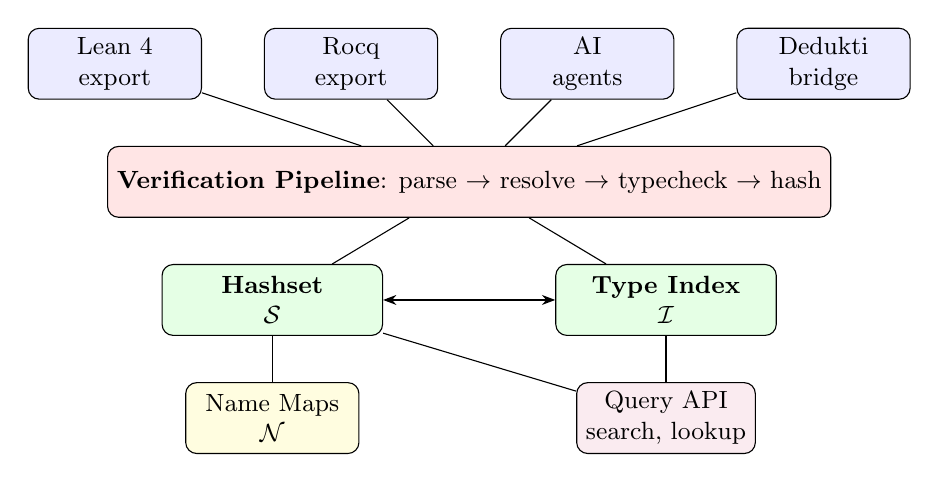
\begin{tikzpicture}[
    component/.style={draw, rounded corners, font=\small, fill=blue!8, minimum width=2.2cm, minimum height=0.9cm, align=center},
    store/.style={draw, rounded corners, font=\small, fill=green!10, minimum width=2.8cm, minimum height=0.9cm, align=center},
    meta/.style={draw, rounded corners, font=\small, fill=yellow!12, minimum width=2.2cm, minimum height=0.9cm, align=center},
    api/.style={draw, rounded corners, font=\small, fill=purple!8, minimum width=2.2cm, minimum height=0.9cm, align=center},
    >=Stealth,
    every edge/.style={draw, ->}
  ]
  % Sources
  \node[component] (lean) at (-4.5, 3) {Lean~4\\export};
  \node[component] (rocq) at (-1.5, 3) {Rocq\\export};
  \node[component] (ai) at (1.5, 3) {AI\\agents};
  \node[component] (ded) at (4.5, 3) {Dedukti\\bridge};

  % Verification
  \node[component, fill=red!10, minimum width=8cm] (verify) at (0, 1.5) {\textbf{Verification Pipeline}: parse $\to$ resolve $\to$ typecheck $\to$ hash};

  % Storage
  \node[store] (hashset) at (-2.5, 0) {\textbf{Hashset}\\$\hashset$};
  \node[store] (typeindex) at (2.5, 0) {\textbf{Type Index}\\$\typeindex$};

  % Metadata
  \node[meta] (names) at (-2.5, -1.5) {Name Maps\\$\namemap$};

  % API
  \node[api] (apiq) at (2.5, -1.5) {Query API\\search, lookup};

  % Edges
  \draw (lean) -- (verify);
  \draw (rocq) -- (verify);
  \draw (ai) -- (verify);
  \draw (ded) -- (verify);
  \draw (verify) -- (hashset);
  \draw (verify) -- (typeindex);
  \draw (hashset) -- (names);
  \draw[<->] (hashset) -- (typeindex);
  \draw (hashset) -- (apiq);
  \draw (typeindex) -- (apiq);
\end{tikzpicture}
\caption{HashMath architecture. Terms from multiple sources pass through the verification pipeline
before being added to the hashset and type index. Name maps are optional metadata. The query API
supports lookup by hash and search by type.}
\label{fig:architecture}
\end{figure}


%% ============================================================
\section{AI and Human Collaboration}
\label{sec:collaboration}

\subsection{The Coordination Problem Today}
\label{sec:coordination-today}

Tao's formalization of the Polynomial Freiman-Ruzsa conjecture in Lean involved over 20
contributors, with manual coordination through GitHub issues, Zulip chat, and personal
communication~\cite{tao2025}.
Mathlib contributions require human review, conformance to naming conventions, and compliance
with style linters.
These processes ensure quality but limit throughput.

AI systems like AlphaProof~\cite{alphaproof} and DeepSeek-Prover-V2~\cite{deepseek}
can produce correct proofs at machine speed, but cannot contribute them to shared
libraries without human intermediation: someone must name the theorem, choose the right
namespace, write documentation, and submit a pull request.
The Polymath project~\cite{gowers2009} demonstrated the vision of permissionless mathematical
collaboration---40+ contributors proving the density Hales-Jewett theorem through blog
comments---but the coordination was entirely ad hoc.

\subsection{HashMath Eliminates Coordination}
\label{sec:no-coordination}

In HashMath, the contribution workflow is:
\begin{enumerate}[nosep]
  \item Agent (AI or human) constructs a well-typed CIC term $t$.
  \item Agent submits $t$ to the hashset.
  \item The verification pipeline checks $t$ and computes $\hash(t)$.
  \item $t$ is available globally, immediately, by hash.
\end{enumerate}

No pull request.
No naming debate.
No review queue.
Another agent that needs a lemma of type $T$ queries $\typeindex(\hash(T))$ and finds $t$
by its type, not by any name.

When multiple agents independently prove the same theorem with the same proof term, they
produce the same hash---the duplicate is automatically detected.
When they produce different proofs of the same theorem, both are stored and discoverable
through the type index.
Neither outcome wastes work.

\subsection{The Naming Layer as Social Convention}
\label{sec:naming-layer}

Names remain useful---for human communication, documentation, textbooks, and teaching.
In HashMath, names are metadata: a mapping from strings to hashes, maintained by communities.

\begin{itemize}[nosep]
  \item The French school: ``th\'eor\`eme de B\'ezout'' $\mapsto$ \texttt{a7f3...}
  \item The English school: ``Bezout's theorem'' $\mapsto$ \texttt{a7f3...}
  \item An AI agent: \texttt{h\_7f3a2b} $\mapsto$ \texttt{a7f3...}
\end{itemize}

All three reference the same hash.
Name collisions are impossible because names are not identity---they are aliases.
Different communities can maintain their own naming conventions without conflict.

\subsection{Scaling Mathematics}
\label{sec:scaling}

Tao's vision of ``big theorems proved by 20 people and multiple AIs'' requires infrastructure
that does not exist today.
HashMath provides it.

Imagine 1000 AI agents exploring different corners of mathematics simultaneously.
Each agent submits verified terms to the hashset.
Other agents discover these terms by type signature and build on them.
Human mathematicians curate, name, and organize the accumulating knowledge---but the raw
content grows permissionlessly, limited only by the rate at which correct proofs can be produced.

\begin{figure}[t]
\centering
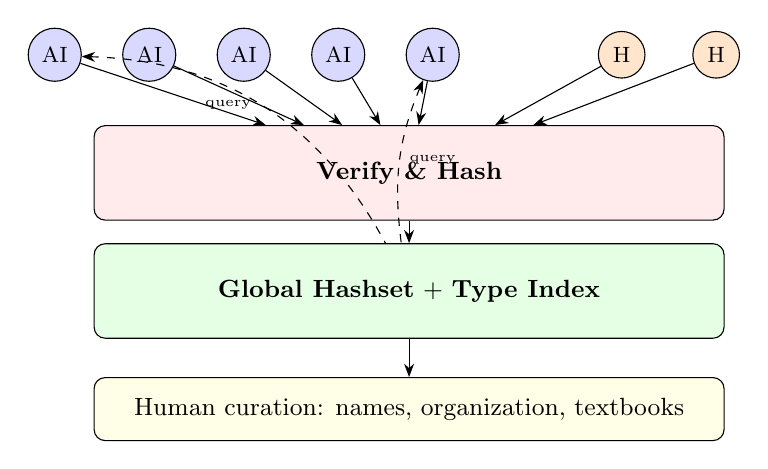
\begin{tikzpicture}[
    agent/.style={draw, circle, inner sep=3pt, fill=blue!15, font=\footnotesize},
    human/.style={draw, circle, inner sep=3pt, fill=orange!20, font=\footnotesize},
    store/.style={draw, rounded corners, fill=green!10, minimum width=3cm, minimum height=1.2cm, align=center, font=\small},
    layer/.style={draw, rounded corners, fill=yellow!10, minimum width=3cm, minimum height=0.8cm, align=center, font=\small},
    >=Stealth
  ]
  % Agents
  \foreach \i in {1,...,5} {
    \node[agent] (a\i) at ({-3 + (\i-1)*1.2}, 2.5) {AI};
  }
  \node[human] (h1) at (4.2, 2.5) {H};
  \node[human] (h2) at (5.4, 2.5) {H};

  % Verification
  \node[store, fill=red!8, minimum width=8cm] (v) at (1.5, 1) {\textbf{Verify \& Hash}};

  % Hashset
  \node[store, minimum width=8cm] (hs) at (1.5, -0.5) {\textbf{Global Hashset} + \textbf{Type Index}};

  % Curation
  \node[layer, minimum width=8cm] (cur) at (1.5, -2) {Human curation: names, organization, textbooks};

  % Edges
  \foreach \i in {1,...,5} {
    \draw[->] (a\i) -- (v);
  }
  \draw[->] (h1) -- (v);
  \draw[->] (h2) -- (v);
  \draw[->] (v) -- (hs);
  \draw[->] (hs) -- (cur);
  \draw[<-, dashed] (a1) to[bend left=30] node[left, font=\tiny] {query} (hs);
  \draw[<-, dashed] (a5) to[bend right=15] node[right, font=\tiny] {query} (hs);
\end{tikzpicture}
\caption{AI agents and humans contribute proof terms to the verification pipeline.
Verified terms enter the global hashset. Agents discover existing results through type-directed queries.
Humans add curation---names, organization, exposition---as an optional layer.}
\label{fig:collaboration}
\end{figure}


%% ============================================================
\section{Challenges and Limitations}
\label{sec:challenges}

We address the principal challenges honestly.

\subsection{Definitional Equality and Hash Diversity}
\label{sec:hash-diversity}

Two CIC terms that are \emph{definitionally equal} but \emph{syntactically different}
receive different hashes.
For example, $(\lambda(x{:}\Nat).\,x)\;\textsf{zero}$ and $\textsf{zero}$ are definitionally
equal but hash differently.
This is by design: the hash captures the exact proof term, not just the proposition it proves.
The type index is the correct mechanism for finding ``equivalent'' results---all proofs of a
given type are discoverable regardless of their syntactic form.

One could normalize terms before hashing to reduce diversity, but normalization is computationally
expensive (exponential in the worst case) and would change the semantics: distinct proof strategies
would become indistinguishable.
We judge that hashing terms as-is, combined with the type index for discovery, is the right tradeoff.

\subsection{Universe Polymorphism}
\label{sec:hash-universes}

Universe-polymorphic definitions are parameterized by universe level variables.
The hash must capture universe parameters correctly: a definition instantiated at $\Type(0)$
and the same definition instantiated at $\Type(1)$ are different terms with different hashes.
The hash function handles this through $\hash_{\textsf{level}}$ and $\hash_{\textsf{levels}}$,
which hash universe level expressions (variables, successors, max) structurally.
Care is needed to ensure that universe constraints are consistently captured.

\subsection{Axiom Compatibility}
\label{sec:axioms}

Different mathematical traditions employ different axioms: classical logic vs.\ constructive logic,
the axiom of choice, propositional extensionality, function extensionality, quotient types, and so on.
In HashMath, axiom dependencies are carried transitively through the Merkle DAG.
Every axiom used in a proof is visible by inspecting the transitive dependencies of its hash.

This enables powerful filtering: ``show me all proofs of $X$ that do not use the axiom of
choice'' is a computable query---walk the Merkle DAG and check whether the axiom of choice's
hash appears in the dependency set.
Different communities can maintain different axiom policies without preventing contribution
to the shared hashset.

\subsection{Hash Stability Across Format Versions}
\label{sec:hash-stability}

If the hashing scheme is ever modified---for example, to add support for a new term
constructor---all hashes change.
The Unison project experienced this challenge in migrating between hash format versions~\cite{unison}.

We mitigate this through several mechanisms:
\begin{itemize}[nosep]
  \item \textbf{Version prefix}: every hash includes a format version byte, so terms self-identify
    their hashing era.
  \item \textbf{Bidirectional mappings}: during transitions, maintain a mapping between old and new hashes.
  \item \textbf{Stability as a goal}: the hash format should be designed carefully and changed rarely.
    Getting it right early is a priority.
\end{itemize}

\subsection{Mutual Recursion}
\label{sec:mutual-challenges}

Block-level hashing (Section~\ref{sec:mutual}) ensures acyclicity but introduces granularity
concerns.
If a mutual block is large, any modification to one definition changes the block hash and
thus the identity of all definitions in the block.
In practice, mutual blocks in CIC tend to be small (2--5 definitions), making this manageable.
Refactoring a mutual block into a non-mutual formulation (when possible) is a content-level
change and correctly results in a different hash.

\subsection{Performance}
\label{sec:performance}

Hashing deep dependency trees requires traversing large Merkle DAGs.
Several standard techniques address this:
\begin{itemize}[nosep]
  \item \textbf{Caching}: once a term's hash is computed, it is stored and never recomputed.
  \item \textbf{Memoization}: shared subterms (which are common in CIC terms) are hashed once.
  \item \textbf{Incremental verification}: when verifying a new term, only the new term and its
    immediate definition need type-checking; dependencies have already been verified.
\end{itemize}

\subsection{Social Adoption}
\label{sec:adoption}

A content-addressed knowledge base is only useful if it contains content.
This is a chicken-and-egg problem with a clear bootstrap strategy:
\begin{itemize}[nosep]
  \item \textbf{Import Mathlib}: Lean~4's Mathlib contains 210,000+ theorems and is CIC-based.
    Importing it provides a substantial initial corpus.
  \item \textbf{AI agent tooling}: provide APIs and tooling that make it easy for AI proving
    systems to submit and query the hashset.
  \item \textbf{Compatibility}: HashMath is complementary to existing systems, not a replacement.
    Lean and Rocq users can continue using their preferred tools; HashMath is the storage and
    discovery layer.
\end{itemize}

\subsection{Eta-Equivalence and Proof Irrelevance}
\label{sec:eta-challenges}

HashMath CIC includes function $\eta$-equivalence ($f \equiv \lambda x.\, f\;x$),
structural $\eta$ for structure-like inductives, and proof irrelevance for $\Prop$.
These features are necessary for compatibility with Lean~4's kernel, but they increase
the complexity of the definitional equality checker and the potential for hash diversity.

Two terms that are $\eta$-equivalent receive different hashes---the hash captures the
exact syntactic structure, not the equivalence class.
However, both terms typecheck against the same type and are therefore both discoverable
through the type index.
This is an intentional design choice: normalizing before hashing would require choosing
a canonical form, which is computationally expensive and may not be unique
for all equivalences.

\subsection{Elaboration Non-Determinism}
\label{sec:elaboration}

Different proof assistants (and different versions of the same assistant) may elaborate
the same mathematical statement into different kernel terms.
Lean~4's tactic mode, for instance, often produces terms with more let-bindings, casts,
and auxiliary definitions than a hand-written proof term.
Since HashMath hashes the \emph{elaborated} term, the same mathematical theorem may receive
different hashes when elaborated by different tools.

This is inherent to any content-addressing scheme that operates below the elaboration level.
The type index mitigates the issue: all proofs of a given type are discoverable regardless
of their elaboration strategy.
Over time, as community norms develop around preferred elaboration patterns, convergence
is expected for core mathematical content.

\subsection{Lean/Rocq Kernel Divergences}
\label{sec:divergences}

While both Lean~4 and Rocq implement CIC, their kernels differ in several important ways:
\begin{itemize}[nosep]
  \item \textbf{Recursors vs.\ match}: Lean~4 uses recursors as the primitive elimination form;
    Rocq uses \texttt{match} expressions.
    These are interdefinable but produce different kernel terms.
  \item \textbf{Quotient types}: Lean includes quotient types as a primitive;
    Rocq constructs them using the axiom of unique choice or via setoid reasoning.
  \item \textbf{Eta rules}: Lean includes function $\eta$ and structural $\eta$ for structures;
    Rocq's definitional equality rules differ slightly.
  \item \textbf{Proof irrelevance}: Lean has proof irrelevance for $\Prop$ at the kernel level;
    in Rocq, this holds only for propositional content in the SProp universe.
  \item \textbf{Literals}: Lean has native literal expressions for natural numbers and strings;
    HashMath CIC eliminates these in favor of \textsf{Nat.zero}/\textsf{Nat.succ} encoding.
  \item \textbf{No \textsf{Set} sort}: Lean does not have Rocq's \textsf{Set} universe.
\end{itemize}
These divergences mean that a theorem elaborated in Lean and the ``same'' theorem elaborated
in Rocq will generally receive different hashes.
Cross-system sharing requires either a translation layer or a shared elaboration pipeline---both
are feasible but represent engineering work beyond the scope of the initial system.

\subsection{Spam, DoS, and Proof Term Bloat}
\label{sec:spam}

An open, permissionless system is vulnerable to spam: adversaries can submit
arbitrarily many well-typed but useless terms (e.g., $\textsf{Nat.succ}^{10^6}(\textsf{zero})$).
This is a \emph{policy} concern, not a specification concern.
Possible mitigations include:
\begin{itemize}[nosep]
  \item \textbf{Size bounds}: reject terms above a configurable size threshold.
  \item \textbf{Rate limiting}: bound the submission rate per identity or IP address.
  \item \textbf{Proof-of-work}: require a computational puzzle alongside each submission.
  \item \textbf{Reputation}: weight search results by community endorsement.
\end{itemize}
None of these mechanisms are part of the CIC specification; they belong to the
policy layer of any deployment.

Relatedly, tactic-elaborated proof terms can be very large---a simple \texttt{omega} call
may expand to thousands of kernel steps.
DAG sharing (deduplicating shared subterms by hash) and compression can significantly
reduce storage costs.
The content-addressed structure naturally enables deduplication: identical subterms that
appear across many proofs are stored exactly once.

\subsection{Axiom Identity Across Systems}
\label{sec:axiom-identity}

Lean's \texttt{propext} (propositional extensionality) and Rocq's propositional extensionality
axiom express the same mathematical principle but, as different kernel terms, receive different hashes.
This means that proofs using Lean's \texttt{propext} and proofs using Rocq's equivalent
cannot share a dependency tree.

Standardizing axiom declarations across systems is future work.
One approach is to define a canonical HashMath CIC declaration for each standard axiom
and require export pipelines to map system-specific axioms to these canonical forms.

\subsection{Type Index Precision}
\label{sec:index-precision}

The type index maps type hashes to inhabitant hashes, using \emph{syntactic} type hashes.
This means that two types that are definitionally equal but syntactically different
(e.g., $\Nat \to \Nat$ and $\Pi(n{:}\Nat).\,\Nat$) produce different index entries.
A query for one will not find inhabitants typed at the other.

Normalizing types before indexing could improve precision but introduces computational cost
and the question of which normal form to use.
In practice, most mathematical types are stated in a relatively canonical form, and
the type index is effective despite this limitation.


%% ============================================================
\section{Related Work}
\label{sec:related}

\subsection{Proof Assistants}

Lean~4~\cite{lean4}, Rocq (formerly Coq)~\cite{coquand1988}, Agda, and Isabelle/HOL
are the dominant proof assistants.
All use named references within curated libraries.
HashMath is complementary: a content-addressed storage layer that any CIC-based system can
read from and write to, without modifying the system itself.

\subsection{Unison}

Unison~\cite{unison} is the closest precedent.
It content-addresses general-purpose functional programs using SHA3 hashes of abstract syntax trees.
HashMath adapts this idea for the Calculus of Inductive Constructions, adding the type-to-inhabitants
index, requiring formal verification before storage, and handling CIC-specific features
(universe polymorphism, inductive types, strict positivity).

\subsection{Logipedia and Dedukti}

The Logipedia project~\cite{logipedia} aims to build a universal library of formal proofs by
translating between systems through the Dedukti logical framework~\cite{dedukti}, based on
the $\lambda\Pi$-calculus modulo theory.
The EuroProofNet COST action~\cite{europroofnet} (2022--2025) has advanced this vision with
over 600 researchers across 47 countries.
Dedukti translates between \emph{different type theories} through a common framework;
HashMath works at the CIC kernel level where Lean and Rocq \emph{already agree}.
The approaches are complementary: Dedukti could translate non-CIC proofs into CIC for
HashMath storage.

\subsection{MetaCoq}

MetaCoq~\cite{metacoq} formalizes the Calculus of Inductive Constructions within Coq itself,
including a verified type checker proved sound with respect to a formal specification.
This demonstrates that the CIC kernel---the core of HashMath's trusted computing base---can
be formally verified.
HashMath could adopt MetaCoq's verified checker to minimize trust assumptions.

\subsection{IPFS and Content-Addressed Storage}

IPFS~\cite{ipfs} provides content-addressed storage for arbitrary data.
HashMath's storage model is similar but domain-specific: it verifies terms before storing them
(IPFS stores any data) and maintains a type index that is meaningful only for CIC terms.
HashMath could use IPFS as an underlying storage layer.

\subsection{Formal Mathematics Libraries}

Mathlib~\cite{mathlib}, the Archive of Formal Proofs, and Rocq's standard library are curated,
centralized, and name-dependent.
They represent enormous investments of human effort.
HashMath is uncurated, decentralized, and name-independent---but can import these libraries
wholesale as its initial corpus.

\subsection{AI for Mathematics}

AlphaProof~\cite{alphaproof}, DeepSeek-Prover-V2~\cite{deepseek}, LeanDojo, and COPRA
produce proofs within existing proof assistants.
HashMath provides a system-agnostic destination for AI-generated proofs, and the type index
provides a natural interface for AI proof search: search by type signature rather than by name.


%% ============================================================
\section{Roadmap}
\label{sec:roadmap}

We outline a phased development plan.

\paragraph{Phase 1: Core Infrastructure.}
Implement the CIC type checker---following Diehl~\cite{diehl200lines}, the core can be realized in
hundreds of lines---the hash function, the hashset with type index, and a canonical binary
serialization format.

\paragraph{Phase 2: Import Pipeline.}
Build a Lean~4 export pipeline that translates \texttt{Expr} to HashMath terms, hashes them,
and populates the hashset.
Import Mathlib as the initial corpus (210,000+ theorems).
Build a Rocq export pipeline for the standard library.

\paragraph{Phase 3: AI Integration.}
Provide an API for AI agents to submit verified terms and query the type index.
Build a type-directed search interface.
Integrate with existing AI proving systems (DeepSeek-Prover, LeanDojo, etc.).

\paragraph{Phase 4: Distribution and Scaling.}
Implement peer-to-peer replication of the hashset.
Optimize incremental syncing (transfer only missing hashes).
Optimize query performance for the type index at scale.

\paragraph{Phase 5: Ecosystem.}
Build IDE integration (VS Code, Emacs) for browsing and searching the hashset.
Build a web interface for exploration.
Support community-maintained name maps.
Develop proof visualization tools.


%% ============================================================
\section{Future Work: Advanced Indices}
\label{sec:indices}

The type-to-inhabitants index (Section~\ref{sec:type-index}) is the simplest
and most fundamental index over the hashset: given a type hash, return all inhabitants.
But a content-addressed knowledge base admits a much richer family of indices, each
enabling a different mode of mathematical search.
We outline several directions.

\subsection{Dependency and Reverse-Dependency Index}
\label{sec:dep-index}

Every declaration's hash transitively encodes its dependencies through the Merkle DAG.
Materializing this as an explicit index yields two maps:
\[
  \textsf{deps}(h) = \{ h' \mid h' \text{ is a transitive dependency of } h \}
\]
\[
  \textsf{rdeps}(h) = \{ h' \mid h \in \textsf{deps}(h') \}
\]
The dependency map answers ``what does this theorem rely on?''---useful for
axiom auditing, minimality checking, and understanding proof structure.
The reverse-dependency map answers ``what builds on this definition?''---essential
for impact analysis and for understanding the downstream consequences of a change.

Both maps are computable from the hashset contents and can be maintained incrementally
as new terms are added.

\subsection{Axiom Filter Index}
\label{sec:axiom-index}

Section~\ref{sec:axioms} noted that axiom dependencies are visible through the Merkle DAG.
A dedicated axiom filter index makes this query efficient:
\[
  \textsf{axioms}(h) = \{ h' \in \textsf{deps}(h) \mid h' \text{ is an axiom} \}
\]
This enables queries like ``find all proofs of $X$ that are constructive'' (no excluded middle),
``find all proofs that avoid the axiom of choice,'' or ``find all proofs
that use only the axioms shared by Lean and Rocq.''
For communities with specific foundational commitments, the axiom filter index
provides automatic compliance checking.

\subsection{Unification-Based Type Search}
\label{sec:unification-index}

The type-to-inhabitants index requires an \emph{exact} type hash match.
This is limiting: the query type must be syntactically identical to the stored type,
modulo alpha-equivalence.
A more powerful search allows the query type to contain metavariables
(wildcards) that are instantiated by unification.

For example, a query for $\forall (n : \Nat),\; ?P\;n \to ?P\;(\textsf{succ}\;n)$
would match any induction step, returning inhabitants whose types unify with the pattern.
This is analogous to Hoogle's type search with polymorphism.

Implementing unification-based search over a large corpus requires indexing techniques
from the term-indexing literature~\cite{graf1996}: discrimination trees, substitution trees,
or path indexing.
Adapting these to CIC terms with dependent types is a nontrivial but tractable
engineering challenge.

\subsection{Head-Symbol Index}
\label{sec:head-index}

Many mathematical queries are about a specific concept: ``find all lemmas about $\textsf{List}$''
or ``find all properties of $\textsf{Ring}$.''
A head-symbol index maps the outermost constant of a type to its inhabitants:
\[
  \textsf{head}(h_c) = \{ h \mid (h, t, T) \in \hashset,\; \textsf{headConst}(T) = h_c \}
\]
where $\textsf{headConst}$ extracts the outermost constant after stripping universal
quantifiers and function arrows.
This is a lightweight approximation to concept-level search, effective for browsing
the knowledge base by topic.

\subsection{Subexpression and Pattern Index}
\label{sec:subexpr-index}

A subexpression index maps each constant hash to the set of terms that mention it:
\[
  \textsf{mentions}(h_c) = \{ h \mid (h, t, T) \in \hashset,\; h_c \text{ occurs in } t \text{ or } T \}
\]
This supports queries like ``find all terms that use $\textsf{Nat.add}$'' or
``find all proofs that apply $\textsf{Eq.trans}$.''
It is a form of full-text search for formalized mathematics.

A more expressive variant allows \emph{pattern matching}: given a template expression
with wildcards, find all terms containing a subexpression matching the pattern.
For example, the pattern $\textsf{Nat.add}\;?\;0$ would find all terms that add zero
to something.
Efficient pattern matching over a large term corpus connects to the literature
on code search and anti-unification.

\subsection{Typeclass and Structure Instance Index}
\label{sec:instance-index}

In systems like Lean~4, typeclass instances are key organizational structures.
A typeclass instance index maps each typeclass (identified by the hash of its
inductive declaration) to the set of instances registered for it:
\[
  \textsf{instances}(h_{\textsf{class}}) = \{ h \mid (h, t, T) \in \hashset,\;
  T \text{ has head constant } h_{\textsf{class}} \}
\]
This enables queries like ``which types have a $\textsf{Group}$ instance?'' or
``find all $\textsf{Monad}$ implementations.''
Combined with the head-symbol index, it supports rich algebraic hierarchy browsing.

\subsection{Normalized Type Index}
\label{sec:norm-index}

Section~\ref{sec:index-precision} noted that the type index uses syntactic type hashes,
so definitionally equal types with different syntax produce different index entries.
A normalized type index addresses this by reducing types to a canonical form before hashing:
\[
  \typeindex_{\textsf{norm}}(h) = \typeindex(\hash(\textsf{normalize}(T)))
  \quad\text{where}\quad \hash(T) = h
\]
The challenge is choosing a normalization strategy.
Full $\beta\delta\iota\zeta$-normalization is computationally expensive (potentially
exponential), but weaker normalizations---such as head-normalizing only the outermost
structure, or normalizing with bounded unfolding depth---may capture most practical
equivalences at acceptable cost.

\subsection{Compositional Search}
\label{sec:compositional}

The indices above can be composed to answer complex queries.
For example:
\begin{itemize}[nosep]
  \item ``Find all constructive proofs of commutativity for rings'':
    unification-based type search for $\forall (R : \textsf{Ring}),\; ?a \cdot ?b = ?b \cdot ?a$,
    filtered by the axiom index to exclude classical axioms.
  \item ``Find all lemmas about $\textsf{List.map}$ that don't depend on $\textsf{Decidable}$'':
    subexpression search for $\textsf{List.map}$, filtered by reverse-dependency exclusion.
  \item ``Find all instances of $\textsf{Functor}$ for types defined in terms of $\textsf{List}$'':
    typeclass instance index for $\textsf{Functor}$, filtered by dependency index for $\textsf{List}$.
\end{itemize}
A query language that supports Boolean combinations of index predicates, analogous to
database query planning, would make the knowledge base into a genuine search engine
for formalized mathematics.


%% ============================================================
\section{Conclusion}
\label{sec:conclusion}

The Calculus of Inductive Constructions is the right foundation for a global mathematical
knowledge base: it is the shared core of the most successful proof assistants, it is
expressive enough for serious mathematics, and its type checker is small enough to be
formally verified.

Content-addressing eliminates the coordination bottleneck that limits the scale of formalized
mathematics.
No naming consensus, no centralized curation, no review queues---just verified terms,
identified by their structure, composable by hash.

The type-to-inhabitants index turns the knowledge base into a searchable library where
AI agents and human mathematicians discover relevant results by type signature, not by
remembering names.

HashMath provides the infrastructure for a future in which thousands of AI agents and hundreds
of mathematicians contribute simultaneously, building on each other's work without a single
naming conflict or a single gatekeeper.

Mathematics should be permissionless.
HashMath makes it so.

\bigskip

\begin{thebibliography}{30}

\bibitem{lean4}
L.~de~Moura and S.~Ullrich,
``The Lean~4 theorem prover and programming language,''
in \emph{Proc.\ CADE-28}, 2021, pp.~625--635.

\bibitem{mathlib}
The Mathlib Community,
``Mathlib4,''
\url{https://github.com/leanprover-community/mathlib4}, 2024.

\bibitem{alphaproof}
AlphaProof and AlphaGeometry Teams,
``AI achieves silver-medal standard solving International Mathematical Olympiad problems,''
\emph{Nature}, 2025.

\bibitem{deepseek}
Z.~Ren et~al.,
``DeepSeek-Prover-V2: Advancing formal mathematical reasoning via reinforcement learning for subgoal decomposition,''
\emph{arXiv:2504.21801}, 2025.

\bibitem{tao2025}
T.~Tao,
``Machine-assisted proofs,''
\emph{ICM Invited Lecture}, 2025.

\bibitem{gowers2009}
W.~T.~Gowers and M.~Nielsen,
``Massively collaborative mathematics,''
\emph{Nature}, vol.~461, pp.~879--881, 2009.

\bibitem{polymath2012}
D.~H.~J.~Polymath,
``A new proof of the density Hales-Jewett theorem,''
\emph{Annals of Mathematics}, vol.~175, no.~3, pp.~1283--1327, 2012.

\bibitem{coquand1988}
T.~Coquand and G.~Huet,
``The Calculus of Constructions,''
\emph{Information and Computation}, vol.~76, pp.~95--120, 1988.

\bibitem{coquand1990}
T.~Coquand and C.~Paulin-Mohring,
``Inductively defined types,''
in \emph{Proc.\ COLOG-88}, LNCS~417, Springer, 1990.

\bibitem{werner1994}
B.~Werner,
``Une th\'eorie des constructions inductives,''
Ph.D.\ thesis, Universit\'e Paris~7, 1994.

\bibitem{paulin1993}
C.~Paulin-Mohring,
``Inductive definitions in the system Coq: Rules and properties,''
in \emph{Proc.\ TLCA}, LNCS~664, Springer, 1993.

\bibitem{diehl200lines}
L.~Diehl,
``Dependent types in 200 lines of Python,''
blog post, 2023.

\bibitem{diehlzoo}
L.~Diehl,
``The Typechecker Zoo,''
\url{https://github.com/larrytheliquid/typecheckerzoo}, 2023.

\bibitem{unison}
P.~Chiusano and R.~Bjarnason,
``Unison: A friendly programming language from the future,''
\url{https://www.unison-lang.org/}, 2024.

\bibitem{merkle1979}
R.~C.~Merkle,
``A certified digital signature,''
in \emph{Proc.\ CRYPTO'89}, LNCS~435, Springer, 1990.
(Original concept, 1979.)

\bibitem{sha3}
NIST,
``SHA-3 Standard: Permutation-based hash and extendable-output functions,''
\emph{FIPS PUB 202}, 2015.

\bibitem{debruijn1970}
N.~G.~de~Bruijn,
``The mathematical language AUTOMATH, its usage, and some of its extensions,''
in \emph{Symposium on Automatic Demonstration}, LNCS~125, Springer, 1970.

\bibitem{pollack1998}
R.~Pollack,
``How to believe a machine-checked proof,''
in \emph{Twenty-Five Years of Constructive Type Theory}, Oxford, 1998.

\bibitem{metacoq}
M.~Sozeau, S.~Boulier, Y.~Forster, N.~Tabareau, and T.~Winterhalter,
``Coq Coq correct! Verification of type checking and erasure for Coq, in Coq,''
\emph{Proc.\ ACM Program. Lang.}, vol.~4 (POPL), pp.~8:1--8:28, 2020.

\bibitem{logipedia}
G.~Dowek,
``Logipedia: a multi-system encyclopedia of formal proofs,''
\emph{arXiv:2305.00064}, 2023.

\bibitem{dedukti}
A.~Assaf, G.~Burel, R.~Cauderlier, D.~Delahaye, G.~Dowek, C.~Dubois, F.~Gilbert, P.~Halmagrand,
O.~Hermant, and R.~Saillard,
``Dedukti: a logical framework based on the $\lambda\Pi$-calculus modulo theory,''
2016.

\bibitem{europroofnet}
F.~Blanqui et~al.,
``EuroProofNet: European research network on digital proofs,''
COST Action CA20111, 2022--2025.

\bibitem{gonthier2008}
G.~Gonthier,
``Formal proof---the Four Color Theorem,''
\emph{Notices of the AMS}, vol.~55, no.~11, pp.~1382--1393, 2008.

\bibitem{gonthier2013}
G.~Gonthier et~al.,
``A machine-checked proof of the Odd Order Theorem,''
in \emph{Proc.\ ITP}, LNCS~7998, Springer, 2013.

\bibitem{leroy2009}
X.~Leroy,
``Formal verification of a realistic compiler,''
\emph{Commun.\ ACM}, vol.~52, no.~7, pp.~107--115, 2009.

\bibitem{ipfs}
J.~Benet,
``IPFS---Content addressed, versioned, P2P file system,''
\emph{arXiv:1407.3561}, 2014.

\bibitem{nakamoto2008}
S.~Nakamoto,
``Bitcoin: A peer-to-peer electronic cash system,''
2008.

\bibitem{buterin2014}
V.~Buterin,
``Ethereum: A next-generation smart contract and decentralized application platform,''
2014.

\bibitem{graf1996}
P.~Graf,
``Term Indexing,''
\emph{Lecture Notes in Computer Science}, vol.~1053, Springer, 1996.

\end{thebibliography}

\end{document}
